\chapter{Experiment}
\label{ch:experiment}

In the Experiment an optical transmitter was simulated in OptSim. The Experiment was divided in three sub-projects.

\section{Project 1}
\label{sec:P1}
For the Experiment an OptiSim Example of a 50~\% RZ-OOK-Transmitter was used. Figure \ref{fig:P1_aufbau} shows this example\footnotemark[3]. In the upper left-hand side theres the PRBS which generates a pseudo-random bit-stream. A logical connection path (green) leads to an NRZ-Rectifier (recnrz1) which generates an electrical output signal. Via an MZI this electrical NRZ-signal gets modulated on a 1550~nm laser. 

Starting in the upper left-hand sinde at the PRBS again, the lower path leads to an divider. Here the DataRate can be divided. In the first project there is no change of the data rate and the divider is 1. 

\begin{figure}%
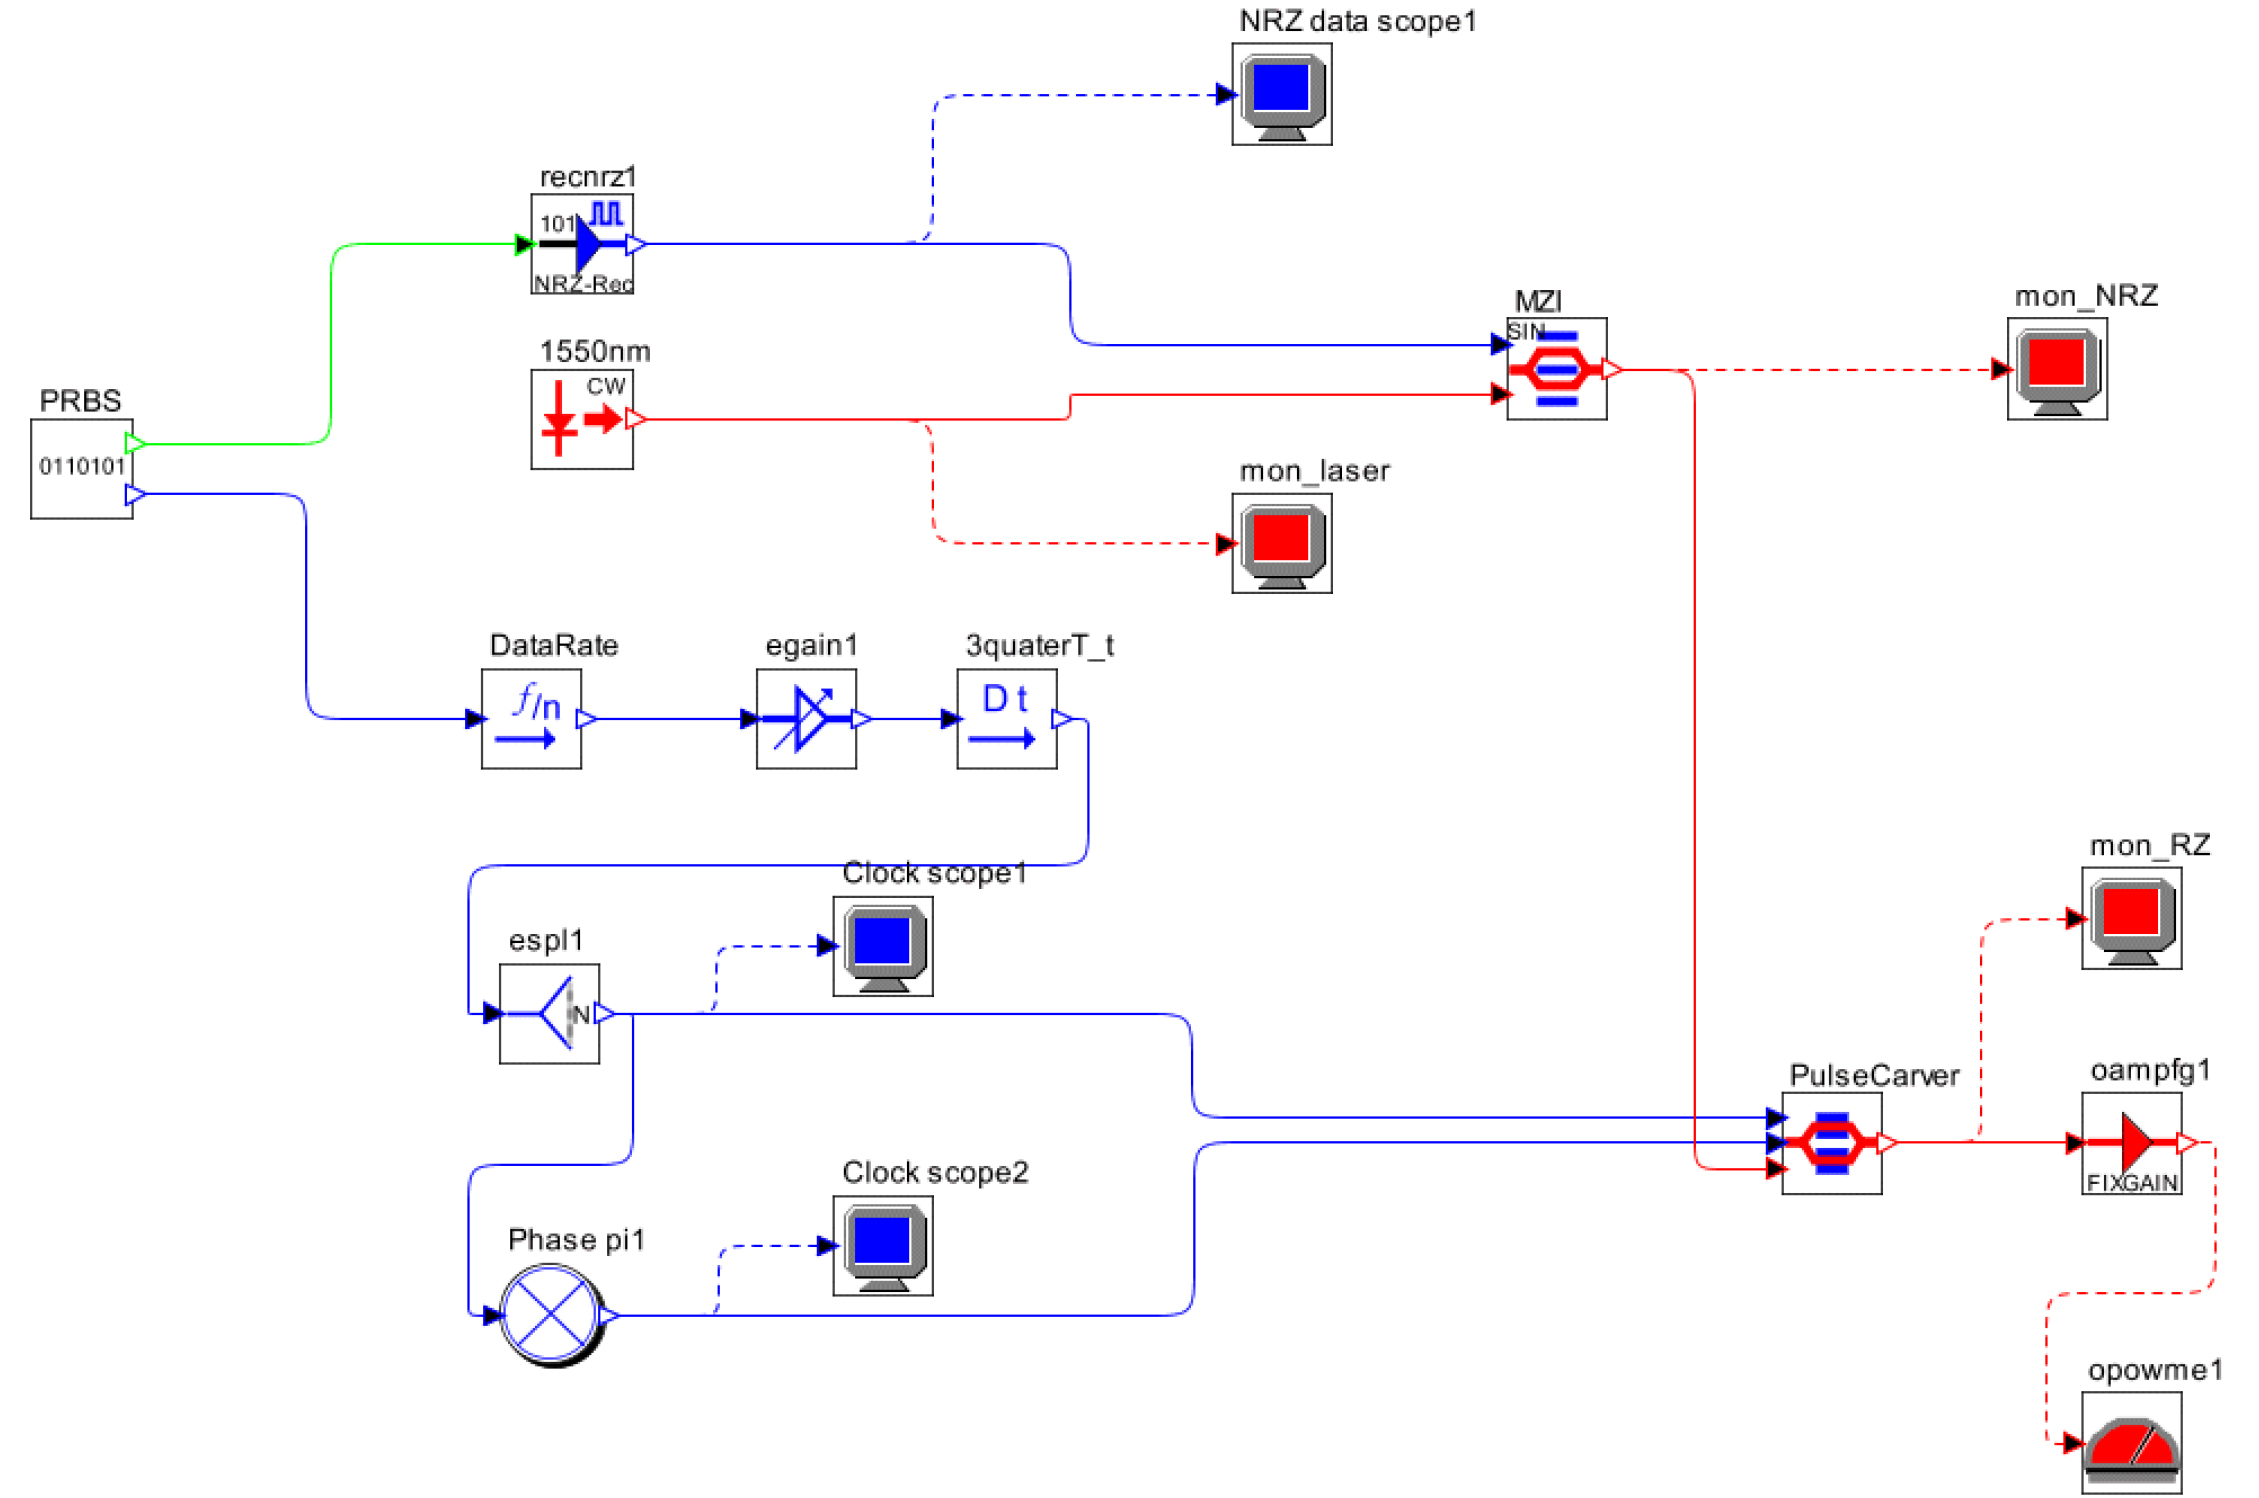
\includegraphics[width=\columnwidth]{Grafiken/P1_aufbau.jpg}%
\caption{OptiSim Sample-Mode example of a 50~\% RZ-OOK-Transmitter}%
\label{fig:P1_aufbau}%
\end{figure}


\footnote[3]{Materials for the Preparation of Experiment 7: Simulation of Optical Transmitters}


\section{Project 2}
In the next Project two PIN photodetectors were inserted. One at the exit of the NRZ-MZM and the other after the optical amplifier("`oampfg1"') for the RZ signal. To display the signal a "`Electrical Monitor"' was placed behind each of the detectors. After running the simulation the eye diagrams of each signal was recorded.

